\documentclass[border=12pt,dvipsnames]{standalone}
\usepackage{pgfplots}
\pgfplotsset{compat=1.17}
\usepackage{xcolor}
\usepackage{tikz}

\definecolor{gold}{HTML}{CFB87C}
\definecolor{dkblue}{HTML}{156082}
\definecolor{ltblue}{HTML}{5B9BD5}
\definecolor{dkgreen}{HTML}{196B24}
\definecolor{ltgreen}{HTML}{70B87C}
\definecolor{dkred}{HTML}{C0392B}
\definecolor{ltred}{HTML}{E07060}
\definecolor{dkgray}{HTML}{333333}
\definecolor{medgray}{HTML}{888888}

\begin{document}
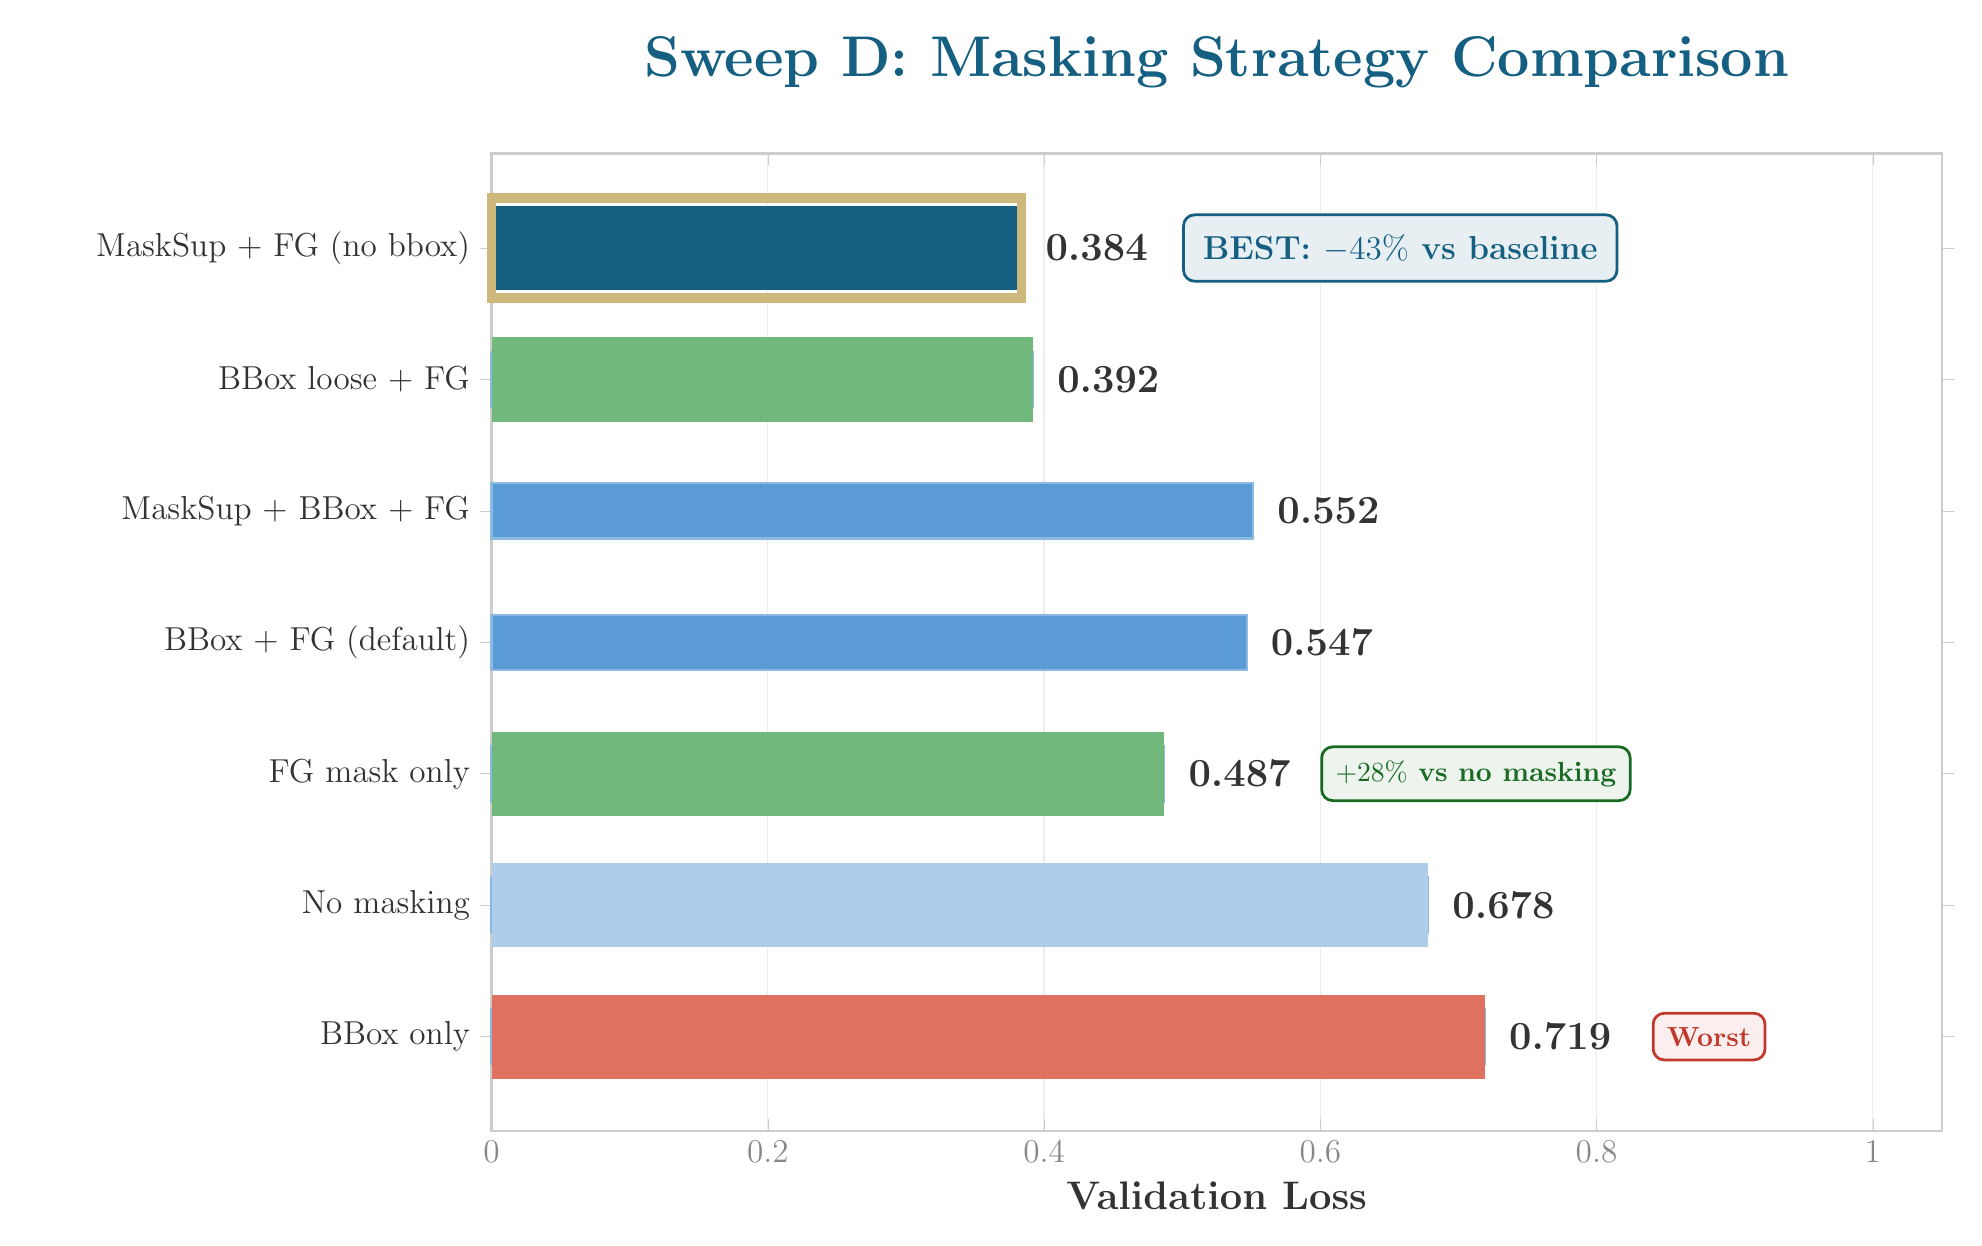
\begin{tikzpicture}
\begin{axis}[
    xbar,
    width=20cm,
    height=14cm,
    bar width=20pt,
    xmin=0, xmax=1.05,
    xlabel={\Large\textbf{Validation Loss}},
    xlabel style={font=\large, color=dkgray},
    title={\huge\bfseries\color{dkblue} Sweep D: Masking Strategy Comparison},
    title style={at={(0.5,1.04)}},
    ytick={0,1,2,3,4,5,6},
    yticklabels={
        {MaskSup + FG (no bbox)},
        {BBox loose + FG},
        {MaskSup + BBox + FG},
        {BBox + FG (default)},
        {FG mask only},
        {No masking},
        {BBox only}
    },
    yticklabel style={font=\large, color=dkgray, align=right, text width=5.5cm},
    xticklabel style={font=\large, color=medgray},
    xtick={0, 0.2, 0.4, 0.6, 0.8, 1.0},
    xmajorgrids=true,
    grid style={gray!15, line width=0.5pt},
    axis line style={gray!40, line width=0.8pt},
    tick style={gray!40},
    nodes near coords,
    every node near coord/.append style={font=\Large\bfseries, anchor=west, xshift=5pt, color=dkgray},
    point meta=explicit symbolic,
    clip=false,
    enlarge y limits=0.12,
    y dir=reverse,
]

% Single addplot with all 7 bars
\addplot[
    xbar,
    fill=ltblue, draw=ltblue!70, line width=0.8pt,
] coordinates {
    (0.3836, 0) [0.384]
    (0.3921, 1) [0.392]
    (0.5515, 2) [0.552]
    (0.5467, 3) [0.547]
    (0.4871, 4) [0.487]
    (0.6782, 5) [0.678]
    (0.7192, 6) [0.719]
};

% Color overlays for specific bars
\fill[dkblue] (axis cs:0, -0.32) rectangle (axis cs:0.3836, 0.32);
\fill[ltgreen] (axis cs:0, 0.68) rectangle (axis cs:0.3921, 1.32);
\fill[ltgreen] (axis cs:0, 3.68) rectangle (axis cs:0.4871, 4.32);
\fill[ltblue!50] (axis cs:0, 4.68) rectangle (axis cs:0.6782, 5.32);
\fill[ltred] (axis cs:0, 5.68) rectangle (axis cs:0.7192, 6.32);

% Gold border on winner
\draw[gold, line width=3.5pt]
    (axis cs:0, -0.38) rectangle (axis cs:0.3836, 0.38);

% Annotations — pushed far right so they don't overlap value labels
\node[fill=dkblue!10, draw=dkblue, rounded corners=4pt, line width=1pt,
      font=\large\bfseries, text=dkblue, inner sep=7pt, anchor=west]
    at (axis cs:0.50, 0) {\textbf{BEST:} $-43\%$ vs baseline};

\node[fill=dkgreen!8, draw=dkgreen, rounded corners=4pt, line width=1pt,
      font=\normalsize\bfseries, text=dkgreen, inner sep=5pt, anchor=west]
    at (axis cs:0.60, 4) {$+28\%$ vs no masking};

\node[fill=dkred!8, draw=dkred, rounded corners=4pt, line width=1pt,
      font=\normalsize\bfseries, text=dkred, inner sep=5pt, anchor=west]
    at (axis cs:0.84, 6) {Worst};

\end{axis}
\end{tikzpicture}
\end{document}
